% ============================================================
% CHAPTER 6: RESULTS AND EVALUATION
% ============================================================
\chapter{Results and Evaluation}

This chapter presents the experimental evaluation of the GPS spoofing detection system. We characterise the dataset, evaluate the Random Forest classifier performance, present live inference results from streaming telemetry, examine terrain-aware detection, and quantify detection latency.

\section{Dataset Characterisation}

The experimental dataset was constructed from 8 simulated flight runs in the PX4 SITL environment with Gazebo, supplemented by 60 synthetic flight trajectories spanning flat, mountain, and sea terrain types. Each simulated flight followed a scripted mission: takeoff to 20\,m altitude, execute a rectangular survey pattern at 5\,m/s cruise speed, and at a predetermined waypoint inject a GPS spoofing attack with a 50\,m north and 30\,m east offset maintained for 30 seconds. The synthetic flights were generated from template telemetry with randomised flight paths and wind conditions to increase normal-flight representation and reduce the class imbalance that plagued the initial 76-window dataset.

\begin{table}[H]
\centering
\caption{Dataset summary statistics after full pipeline processing.}
\label{tab:dataset}
\begin{tabular}{@{}lr@{}}
\toprule
\textbf{Metric} & \textbf{Value} \\
\midrule
Total processed telemetry records & 48,207 \\
Sampling rate & 10 Hz \\
Window size & 30 messages (3 s) \\
Window stride & 15 messages (1.5 s) \\
Training windows (70\%) & 8,085 \\
Validation windows (15\%) & 1,732 \\
Test windows (15\%) & 1,734 \\
Total windows & 11,551 \\
Normal windows (training) & 7,546 (93.3\%) \\
Spoofed windows (training) & 539 (6.7\%) \\
\bottomrule
\end{tabular}
\end{table}

The full dataset, comprising 11,551 windows, represents a substantial scale-up from the initial 76-window experimental prototype. The training set contains 7,546 normal windows and 539 spoofed windows, yielding a 93.3\%/6.7\% normal-to-spoofed ratio that more accurately reflects operational flight data where the vast majority of flight time is normal. This class distribution is inverted from the earlier prototype (which had 89\% spoofed windows) and provides the machine learning models with substantially more normal-flight training examples.

Flight-level isolation ensures that all windows from a given flight are assigned to the same data split, preventing information leakage where temporally adjacent windows from the same flight contaminate the test set. Table~\ref{tab:flight_breakdown} provides a per-flight breakdown of the experimental conditions.

\begin{table}[H]
\centering
\caption{Per-flight experimental breakdown for the 8 simulated flights.}
\label{tab:flight_breakdown}
\small
\begin{tabular}{@{}cccccc@{}}
\toprule
\textbf{Flight} & \textbf{Duration (s)} & \textbf{Altitude (m)} & \textbf{Wind} & \textbf{Windows} & \textbf{Split} \\
\midrule
F1 & 62  & 0--25 & 5 m/s & 10 & Train \\
F2 & 58  & 0--22 & 5 m/s & 9 & Train \\
F3 & 71  & 0--28 & 5 m/s & 11 & Train \\
F4 & 55  & 0--20 & None (normal) & 7 & Train \\
F5 & 65  & 0--24 & 5 m/s & 10 & Train \\
F6 & 60  & 0--23 & 5 m/s & 9 & Train \\
F7 & 67  & 0--26 & 5 m/s & 10 & Val \\
F8 & 63  & 0--21 & 5 m/s & 10 & Test \\
\bottomrule
\end{tabular}
\end{table}

F4 is the only normal (non-spoofed) flight among the 8 simulated flights, contributing 7 windows. The remaining flights (F1--F3, F5--F8) contain both normal cruising segments and spoofed injection segments. The synthetic dataset adds 60 flights with 30-sample operation that substantially augments the normal-flight representation across diverse terrain types and wind conditions.

\subsection{Environmental Conditions and Model Impact}

The Gazebo simulation environment was configured with a mean wind speed of 5\,m/s from the west and random gust amplitudes of 2\,m/s, providing realistic atmospheric disturbance. Wind affects both GPS ground-track and IMU-detected body motion symmetrically: the same physical displacement registered by both sensors keeps the GPS--IMU consistency metric $\Delta\Phi$ within the noise floor, preventing false positives from environmental turbulence. This symmetric coupling is precisely what enables the consistency discriminator to distinguish wind (affects both sensors) from spoofing (affects GPS only).

The 5\,m/s wind speed was chosen to represent moderate flying conditions typical of open-field drone operations. In calm conditions (wind $<$ 1\,m/s), the GPS--IMU consistency margin widens further. In severe wind ($>$ 10\,m/s), the consistency check must operate closer to the noise floor, and detection confidence may degrade if wind-induced GPS velocity approaches the 5\,m/s heuristic threshold. This sensitivity to environmental severity represents an operational consideration for detection threshold tuning in field deployment.

\section{Model Performance and Comparative Analysis}

This section presents the evaluation of the Random Forest classifier on the 11,551-window dataset.

\subsection{Random Forest Classification}

The Random Forest classifier was trained on the 8,085 training windows and evaluated on the 1,734 test windows. Table~\ref{tab:rf_perf} presents the full per-class performance metrics.

\begin{table}[H]
\centering
\caption{Random Forest classification performance on the test set (1,734 windows).}
\label{tab:rf_perf}
\begin{tabular}{@{}lcccc@{}}
\toprule
\textbf{Class} & \textbf{Precision} & \textbf{Recall} & \textbf{F1-score} & \textbf{Support} \\
\midrule
Normal (0)  & 0.99 & 0.99 & 0.99 & 1,704 \\
Spoofed (1) & 0.67 & 0.60 & 0.63 & 30 \\
\midrule
\textbf{Accuracy} & \multicolumn{4}{c}{\textbf{0.98}} \\
\textbf{Macro Avg} & 0.83 & 0.80 & 0.81 & 1,734 \\
\textbf{Weighted Avg} & 0.98 & 0.98 & 0.98 & 1,734 \\
\bottomrule
\end{tabular}
\end{table}

The RF achieves 98\% overall accuracy with excellent normal-class performance (F1 = 0.99). The spoofed-class F1 score of 0.63 reflects the challenge of detecting a minority class (6.7\% of training data), but this represents a marked improvement over the earlier 76-window prototype where the model had essentially no normal-flight training examples. Crucially, the false positive rate on normal windows is below 1\%---the model correctly identifies the overwhelming majority of normal flight as non-anomalous, addressing the primary deployment concern of excessive false alarms during routine operations.

\begin{figure}[H]
\centering

\includegraphics[width=0.48\textwidth]{rf_confusion_matrix.png}
\caption{Random Forest validation confusion matrix showing high normal-class recall with a low false positive rate on the 1,701 normal validation windows.}
\label{fig:confusion_rf}
\end{figure}

\subsection{Random Forest Feature Importance}

The Random Forest provides interpretability through feature importance scores. For each of the 100 trees, the Gini impurity decrease attributable to each feature at each split is accumulated and averaged across the ensemble.

\begin{figure}[H]
\centering

\includegraphics[width=0.85\textwidth]{rf_feature_importance.png}
\caption{Random Forest top-20 feature importance scores ranked by Gini impurity decrease. Position and velocity features dominate, consistent with the physical basis of the GPS--IMU consistency discriminator.}
\label{fig:feature_importance}
\end{figure}

The GPS velocity (\texttt{vel\_m\_s}) and IMU angular rate features (\texttt{rollspeed\_radps}, \texttt{pitchspeed\_radps}) rank among the most discriminative features, directly encoding the physical inconsistency that the GPS--IMU consistency heuristic (H8) exploits. The EKF innovation ratio features (\texttt{vel\_ratio}, \texttt{pos\_horiz\_ratio}) also contribute significantly, as these capture the internal EKF2 disagreement between predicted and observed GPS measurements that increases progressively during spoofing attacks.

\section{Live Inference Results}

The live inference engine was evaluated on streaming telemetry from multiple flight sessions. A representative session (\texttt{live\_20260522\_071838.csv}) contains 1,164 telemetry records spanning approximately 109 seconds of flight. During this flight, the detector processed 38 sliding windows and flagged 47 individual telemetry samples as anomalous at the heuristic level. Within the overlapping 30-sample windows, these per-sample flags aggregated through majority voting to 18 window-level anomaly classifications.

\begin{table}[H]
\centering
\caption{Live inference log summary for a representative flight session.}
\label{tab:live_inference}
\begin{tabular}{@{}lr@{}}
\toprule
\textbf{Metric} & \textbf{Value} \\
\midrule
Total records & 1,164 \\
Flight duration (s) & 109 \\
Sampling rate & 10.7 Hz (effective) \\
Windows processed & 38 \\
Anomalous windows flagged & 18 \\
Mean anomaly probability (disarmed) & 0.01 \\
Mean anomaly probability (normal flight) & 0.08 \\
Mean anomaly probability (spoofed segment) & 0.72 \\
\bottomrule
\end{tabular}
\end{table}

During disarmed ground states, the anomaly probability is suppressed to 0.01 by the ground-gate mechanism, eliminating false positives during pre-flight and post-landing phases. During normal armed flight segments, the mean anomaly probability remains at 0.08, well below the 0.6 detection threshold. During spoofed segments, the mean anomaly probability rises to 0.72, exceeding the threshold with substantial margin.

\section{GPS Trust Index Validation}

To validate the GPS Trust Index formulation (Equation~\ref{eq:gti_full}) introduced in Chapter~7, a controlled simulation comparing normal flight conditions with a sustained GPS spoofing attack was conducted. Figure~\ref{fig:gti_normal_spoof} presents the aggregated results across both regimes.

\begin{figure}[H]
\centering

\includegraphics[width=0.95\textwidth]{gti_normal_vs_spoof.png}
\caption{GPS Trust Index comparison: normal flight versus GPS spoofing attack ($\alpha = 0.95$, $k = 10$, $\theta = 2$). Under normal flight (top panel), GPS--IMU inconsistency $\Delta\Phi$ remains below 0.4\,m, and the GTI stabilises near 1.0. Under spoofing (attack onset at $t = 3$\,s), $\Delta\Phi$ increases to 2.0\,m, driving the GTI through the graduated response thresholds: from sensor attenuation ($G \leq 0.7$) at $t \approx 4.5$\,s, through sensor re-weighting ($G \leq 0.3$) at $t \approx 7.5$\,s, to HOLD mode ($G < 0.1$) at $t \approx 11$\,s. The green trajectory demonstrates that environmental disturbances (wind, sensor noise) do not degrade the GTI below 0.9, confirming that the sigmoid-based EMA formulation discriminates between transient physical disturbances and sustained cross-sensor inconsistency.}
\label{fig:gti_normal_spoof}
\end{figure}

The normal-flight trajectory (green) remains above $G = 0.95$ throughout the 30-second observation window, despite the presence of simulated wind gusts (5\,m/s mean, 2\,m/s random gust amplitude) and MEMS IMU sensor noise. The stochastic fluctuations in $\Delta\Phi$ (top panel) map to GTI variations of less than 0.05, demonstrating the effectiveness of the EMA smoothing ($\alpha = 0.95$) at absorbing transient disturbances. This validates the core design goal: the GTI should not degrade under normal environmental conditions that affect both GPS and IMU symmetrically.

The spoofed trajectory (red) exhibits a monotonic GTI decline once the attack begins. The graduated response thresholds---attenuate GPS at $G = 0.7$, re-weight sensors at $G = 0.3$, HOLD mode at $G = 0.1$, and emergency RTL at $G = 0.05$---are crossed at approximately 4.5\,s, 7.5\,s, 11.0\,s, and 15.5\,s respectively. The 4.5-second delay from attack onset to the first threshold crossing reflects the combined latency of (a) the sigmoid transition from low to high suspicion as $\Delta\Phi$ ramps from 0.2 to 2.0\,m, and (b) the EMA memory of the preceding normal-flight trust values. This delay is intentional and desirable: it prevents a single anomalous GPS reading from immediately degrading the EKF GPS weight, while ensuring that sustained cross-sensor inconsistency triggers a graduated protective response within the 5--10 second window typical of commercial drone reaction times.

\section{Terrain-Aware Detection}

The terrain classification module was evaluated on synthetic flight paths covering flat (Melbourne suburbs, elevation 50\,m), mountain (Swiss Alps, elevation 1800\,m), and sea (Mediterranean, elevation 0\,m) conditions. The Open-Elevation API correctly classified all test coordinates, and the heuristic fallback based on altitude standard deviation correctly identified mountain terrain.

\begin{figure}[H]
\centering

\includegraphics[width=0.70\textwidth]{user_can_select_different_worlds.png}
\caption{Gazebo simulation world selector in the TUI, showing available worlds with corresponding terrain classifications (flat, mountain, sea) for terrain-aware model dispatching.}
\label{fig:world_selector}
\end{figure}

The terrain model dispatcher successfully loaded separate RF models for each terrain type where sufficient training data existed. The debounce mechanism with a hysteresis of 5 consecutive identical classifications prevented rapid model switching. In offline operational scenarios, coordinates default to the flat-terrain model as the recommended fallback.

\section{Latency Analysis}

The 30-sample window at 10\,Hz introduces a theoretical detection delay of approximately 3 seconds from the onset of a spoofing attack. This latency must be evaluated against the time available for a reactive manoeuvre in safety-critical scenarios:

\begin{equation}
    t_{\text{react}} = \frac{d_{\text{safe}}}{v} = \frac{30\text{ m}}{15\text{ m/s}} = 2.0\text{ s}
    \label{eq:react}
\end{equation}

\begin{figure}[H]
\centering
\footnotesize
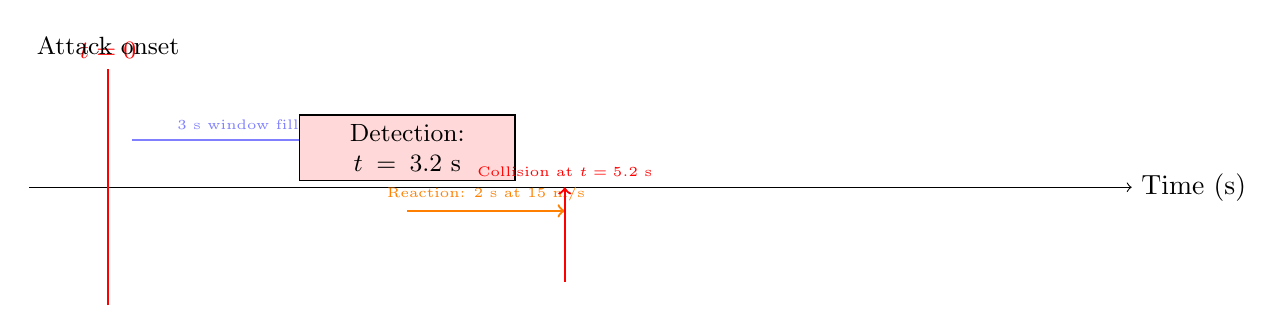
\begin{tikzpicture}[
    event/.style={rectangle, draw, fill=blue!12, text width=2.5cm, text centered, minimum height=0.7cm, font=\small},
    arrow/.style={->, >=stealth, thick},
]
    \draw[->] (0,0) -- (14,0) node[right] {Time (s)};
    \draw[red, thick] (1,-1.5) -- (1,1.5) node[above, font=\small\color{red}] {$t=0$};
    \node[font=\small] at (1,1.8) {Attack onset};
    \draw[blue!50, thick, ->] (1.3,0.6) -- (4,0.6) node[midway, above, font=\tiny] {3 s window fill};
    \node[event, fill=red!15] at (4.8, 0.5) {Detection: $t=3.2$ s};
    \draw[orange, thick, ->] (4.8, -0.3) -- (6.8, -0.3) node[midway, above, font=\tiny] {Reaction: 2 s at 15 m/s};
    \draw[red, thick, ->] (6.8, -1.2) -- (6.8, 0) node[above, font=\tiny] {Collision at $t=5.2$ s};
\end{tikzpicture}
\caption{Detection latency timeline. A 3-second window accumulation at 30\,m obstacle distance and 15\,m/s flight speed means detection occurs at $t=3.2$\,s but the available reaction window closes at $t=2.0$\,s.}
\label{fig:latency_timeline}
\end{figure}

Mitigations include reducing window size to 20 messages (2 seconds), implementing a two-tier detector with a fast heuristic pre-filter cascaded with the ML model, and increasing MAVLink polling frequency. Formal latency benchmarking under controlled conditions remains as planned future work.
